\documentclass[10pt]{article}
\usepackage[preprint]{rlj}
\usepackage{graphicx,booktabs}
\title{Reinforcement Learning Assignment\\ARC-AGI-3: Interactive Reasoning Agents}
\setrunningtitle{WitsC: DQN and PPO for ARC-AGI-3}
\author{Nathan Le Roux, Tafara Chibanda, Samuel Snyman, Joshua Snyman}
\emails{\{2717495,2683459,2677730,2677722\}@students.wits.ac.za}
\affiliations{University of the Witwatersrand --- COMS4061A/COMS7071A}
\begin{document}
% No makeCover: the course disables the RLC cover page.
\maketitle
\begin{abstract}
We investigate convolutional DQN and PPO agents for the interactive puzzles of ARC-AGI-3 under a limited training budget. Both agents share an interface that represents four visual frames and a discrete click lattice. We test episodic novelty and action-history interventions separately for each algorithm. On one development game, sampled PPO with novelty completes a level in 28/60 evaluation episodes, compared with 5/60 for its baseline. DQN with 30\% evaluation exploration completes a level in 42/60 baseline episodes; novelty and memory each reduce this, while their combination reaches 45/60. Neither algorithm solves a full game. Visual replay shows that the original action representation cannot reach any second-level tile. A finer grid restores reachability but does not improve first-level completion under the same budget. Under the official RHAE metric, computed locally, the best trained condition scores 0.36\% on ft09 and every held-out score is below 0.01\%. These results separate policy activity, exploration and representational feasibility from reliable reasoning. Code: \url{https://github.com/TafaraC/RL_Project}.
\end{abstract}

\section{Problem and research questions}
ARC-AGI-3 requires an agent to infer unfamiliar controls and goals through sequential interaction with visual games \citep{arcagi3,arc2026}. The agent receives public observations and legal actions, but no rules and no complete latent state. We ask three questions. Can modest reinforcement-learning agents discover useful behaviour? Do novelty and short memory improve it? Does the action representation itself prevent progress? We do not propose a new algorithm or a general puzzle solver.

DQN is the value-based algorithm covered in the course; PPO is the policy-gradient algorithm not covered in the course. Both share a scaffold built on PyTorch \citep{paszke2019}, NumPy \citep{harris2020} and Gymnasium \citep{towers2024}; the novelty, reset, rollout-memory and inference logic were written and tested for this project. Related methods are DQN's replay and target network \citep{mnih2015}, PPO's clipped objective \citep{schulman2017} and generalized advantage estimation \citep{schulman2016}. Our novelty bonus follows count-based exploration \citep{strehl2008,bellemare2016}, using exact frame counts rather than a learned density model. Learned curiosity signals, such as prediction error in a learned feature space \citep{pathak2017} or random network distillation \citep{burda2019}, extend this idea to large state spaces. Exact counts suffice here because ARC frames are discrete and repeat exactly.

\section{Environment formulation and interface}
The game is partially observable. The four-frame history approximates the state; it is not a proven Markov state. Each 64-by-64 frame has 16 colour indices, encoded as 16 one-hot planes. Four post-action frames give 64 input channels, with missing history zero-padded. Only the newest frame of each response is appended. Engine internals are never used as policy features.

Seven simple actions (RESET, ACTION1--5 and ACTION7) and an $8\times8$ lattice of click centres give 71 actions. ACTION6 carries click coordinates; when it is legal, all lattice cells are legal. The finer $16\times16$ lattice gives 263 actions. Action masks come from the public interface. Discretisation keeps the action space small but can remove necessary actions.

The Gymnasium adapter returns the latest frame, the action mask and progress information. WIN terminates an episode; 1,000 consumed actions truncate it. GAME\_OVER triggers a reset inside the same episode, clearing visual and action history while keeping the agent's parameters. The initial reset is excluded from the budget; internal resets count. A chosen RESET also clears history. The official framework counts the initial reset, so the notebook allows 1,001 calls in total. Training decisions and consumed actions therefore differ.

Training reward is $+1$ per completed level, $+5$ on WIN, $-0.05$ on death and $-0.002$ per action. These rewards are for learning only. We report two evaluation measures, both including unsuccessful episodes: level completion, and the official relative human action efficiency (RHAE) score computed locally (Section~5.3).

\section{Learning algorithms}
\subsection{DQN}
DQN learns an action-value function $Q_\theta(h,a)$ from replayed transitions. The masked Bellman target is $y=r+\gamma(1-d)\max_{a'\in\mathcal A(h')}Q_{\bar\theta}(h',a')$, with a separate target network and Huber loss. True terminals stop bootstrapping; action-budget truncation keeps it. Epsilon-greedy behaviour explores legal actions during training. Network parameters persist across episodes. Replay is used only in training. The target network is copied periodically to stabilise learning.

The CNN has three convolutional layers with 32, 64 and 64 channels, kernels 5, 3 and 3 and stride 2, followed by a 512-unit fully connected layer and the action outputs. Adam \citep{kingma2015} learning rate is $2.5\times10^{-4}$, discount 0.99, batch size 64 and replay capacity 10,000 transitions. Learning starts after 1,000 transitions, updates occur every four decisions and the target is copied every 1,000 gradient updates. Epsilon decays from 1 to 0.05 over 50,000 decisions. Observations are bit-packed to limit replay memory. Run configurations are stored with the evidence.

\subsection{PPO and its update loop}
PPO learns a categorical policy and a scalar value on the same CNN, with one extra value output. During training it samples a legal action and stores the observation, mask, old log probability, reward and value. After 128 transitions, generalized advantage estimation computes
\begin{equation}
\delta_t=r_t+\gamma V(h_{t+1})-V(h_t),\qquad
\hat A_t=\delta_t+\gamma\lambda\hat A_{t+1},
\end{equation}
with terminal, bootstrap and reset-boundary masks applied separately. True terminals use zero next value; truncations bootstrap but stop advantage recursion across episode resets. Advantages are normalised over the rollout.

With $\rho_t=\pi_\theta(a_t|h_t)/\pi_{\mathrm{old}}(a_t|h_t)$, PPO minimises the negative mean of $\min(\rho_t\hat A_t,\mathrm{clip}(\rho_t,0.8,1.2)\hat A_t)$, plus $0.5$ times the value mean-squared error, minus $0.01$ times the policy entropy. Each update runs four epochs over minibatches of 32. Adam learning rate is $3\times10^{-4}$, $\gamma=0.99$, $\lambda=0.95$ and the gradient norm is capped at 0.5. Old masks and probabilities stay fixed during each update. Rollouts store the exact augmented observations, so a history intervention cannot change the likelihood-ratio inputs. The partial final rollout is used for one last update before saving.

Evaluation freezes all weights. PPO samples from its policy; greedy evaluation is a secondary diagnostic. DQN is evaluated with epsilon 0.3, chosen after inspecting development behaviour. Exploration is therefore part of the evaluated DQN policy, and the choice carries selection bias. We do not compare greedy DQN with sampled PPO as if they used the same decision rule.

\section{Experimental protocol}
A recorded shuffle (seed 2026) of the 25 public games selects dc22, ft09, g50t and m0r0 for development and reserves cd82, tr87 and vc33 for final transfer. Each development game is trained separately with independent training seeds 0, 1 and 2 and a target of 50,000 decisions. The runner finishes its last episode, so each run uses about 50,600--51,000 decisions. PPO checkpoints are evaluated for 20 rollouts with sampling seeds 100--119 and 1,000 actions. Stochastic DQN evaluations on ft09 also use 20 rollouts. Older stochastic DQN evaluations on dc22, g50t and m0r0 use ten per checkpoint, so those comparisons have unequal evaluation sample sizes. These seeds control action selection, not game layouts.

The main comparison has three DQN stages, a combined DQN ablation on ft09 and five PPO conditions. Each seed is an independently trained model; the 60 pooled rollouts per condition are not 60 independent models. We therefore report per-seed results rather than significance tests. Development evaluations reuse training games and cannot establish generalisation. The random reference runs seeds 0--2 for 20 episodes per development game. It completes a ft09 level in 2, 5 and 8 episodes and none on the other games. An earlier ft09-only random run with a different random-number schedule gave 5, 9 and 8.

PPO was trained on Windows with Python 3.14.3, PyTorch 2.14.1+cu130 and an RTX 3050 Laptop GPU. DQN improvement runs used Python 3.12.10 on the CPU. Both used arcengine 0.9.3 and arc-agi 0.9.9. The game engine runs on the CPU in both cases. Because hardware differs, elapsed time is not a clean measure of algorithmic efficiency.

\section{Iterative improvements and development evidence}
\subsection{DQN: exploration and no-change memory}
The baseline's greedy policy repeatedly selects a few actions. Training-time completions may therefore come from exploration noise rather than from a capable greedy policy. The first improvement adds a training-only first-visit screen bonus of 0.01, capped at 0.5 per episode, to encourage visual exploration. It does not help: ft09 completion falls from 42/60 to 13/60. The evaluation logs show repeated ineffective actions. The greedy novelty policy on ft09 (one greedy episode per seed) spends 99.4\% of its actions on moves that leave the screen unchanged, repeats a single action for 99.3\% of all actions and sees about seven distinct screens per episode. An unchanged screen earns no first-visit bonus. The bonus did not prevent these loops, although the logs alone do not explain why the policy continued to choose those actions.

The second improvement targets this failure directly. A per-screen memory records actions that left the latest frame unchanged and masks them when the agent returns to that screen. If every legal action would be masked, the full legal mask is restored. The memory uses public screen history, lasts for one episode and changes action selection without a learned recurrent model.

The memory-only condition disables novelty, isolating the memory from the bonus that preceded it. It changes the behaviour it targets: the greedy memory-trained policy on ft09 repeats its most frequent action for 21\% of actions, with 62\% unchanged-screen actions, against 99\% for both after novelty. Breaking the loop does not by itself produce more completions. The combined novelty-plus-memory checkpoints are evaluated on ft09 under the same 20-rollout, epsilon-0.3 protocol. Seeds 0, 1 and 2 clear a level in 19, 8 and 18 episodes (45/60). This exceeds novelty alone (13/60) and memory alone (25/60), but only slightly exceeds the baseline (42/60), with large seed variation. The combined condition was trained on ft09 only and is not part of the transfer comparison. Applying memory at evaluation time to the baseline DQN gives 47/60; this diagnostic does not show a benefit of training with memory. Earlier DQN evaluations did not save their configurations, so their epsilon and memory settings are taken from directory names and scripts.

\subsection{PPO: novelty, then explicit action history}
Baseline sampled PPO rarely completes the first ft09 level. We add a diminishing bonus $0.01/\sqrt{N(s)}$ for the exact newest screen, capped at 0.5 per episode. Counts persist across internal death resets and reset at the next episode. Unlike DQN's first-visit bonus, repeated screens keep a decreasing reward. Pooled ft09 level completion rises from 5/60 to 28/60, but seed 2 dominates the result with 20/20, against 4/20 for each other seed.

Visual diagnosis motivates the second intervention: explicit history of previous actions, repeated actions and unchanged screens. Sixteen binary planes encode the previous simple action (seven planes), the previous click cell (one) and two four-step saturating counters (eight). They are prepended to the four visual frames, giving 80 channels. Memory clears on reset and continues across level transitions. The reward and PPO objective are unchanged. A finer-grid novelty-only control isolates the effect of memory, and a memory-only condition removes novelty. Memory plus novelty reaches 3/60, against 10/60 for the matched control; memory alone reaches 6/60. This intervention does not help. Our hypothesis is a budget effect, not isolated here: the 16 extra planes and the 263-action grid enlarge both the policy's input and its output under the same 50,000-decision budget, so there is more to learn from equally sparse successes. A longer budget for the 16-by-16 conditions would test this.

\begin{table}[t]
\centering
\caption{ft09 frozen development evaluation. Each seed column is successful episodes out of 20; success means at least one completed level. DQN uses epsilon 0.3, PPO samples from its policy and random uses uniform legal actions. The last column is the mean and standard deviation of the three seeds' success rates. No condition wins the full game.}
\begin{tabular}{lrrrr}
\toprule Condition & Seed 0 & Seed 1 & Seed 2 & Mean $\pm$ SD (\%) \\
\midrule Random reference &2&5&8&25.0 $\pm$ 15.0\\
DQN baseline &17&20&5&70.0 $\pm$ 39.7\\
DQN novelty &7&1&5&21.7 $\pm$ 15.3\\
DQN no-change memory &3&17&5&41.7 $\pm$ 37.9\\
DQN novelty + memory &19&8&18&75.0 $\pm$ 30.4\\
DQN baseline + evaluation-time memory &19&20&8&78.3 $\pm$ 33.3\\
PPO baseline, grid 8 &2&0&3&8.3 $\pm$ 7.6\\
PPO novelty, grid 8 &4&4&20&46.7 $\pm$ 46.2\\
PPO novelty, grid 16 control &0&9&1&16.7 $\pm$ 24.7\\
PPO memory + novelty, grid 16 &1&1&1&5.0 $\pm$ 0.0\\
PPO memory only, grid 16 &2&0&4&10.0 $\pm$ 10.0\\
\bottomrule
\end{tabular}
\label{tab:results}
\end{table}

\begin{figure}[t]
\centering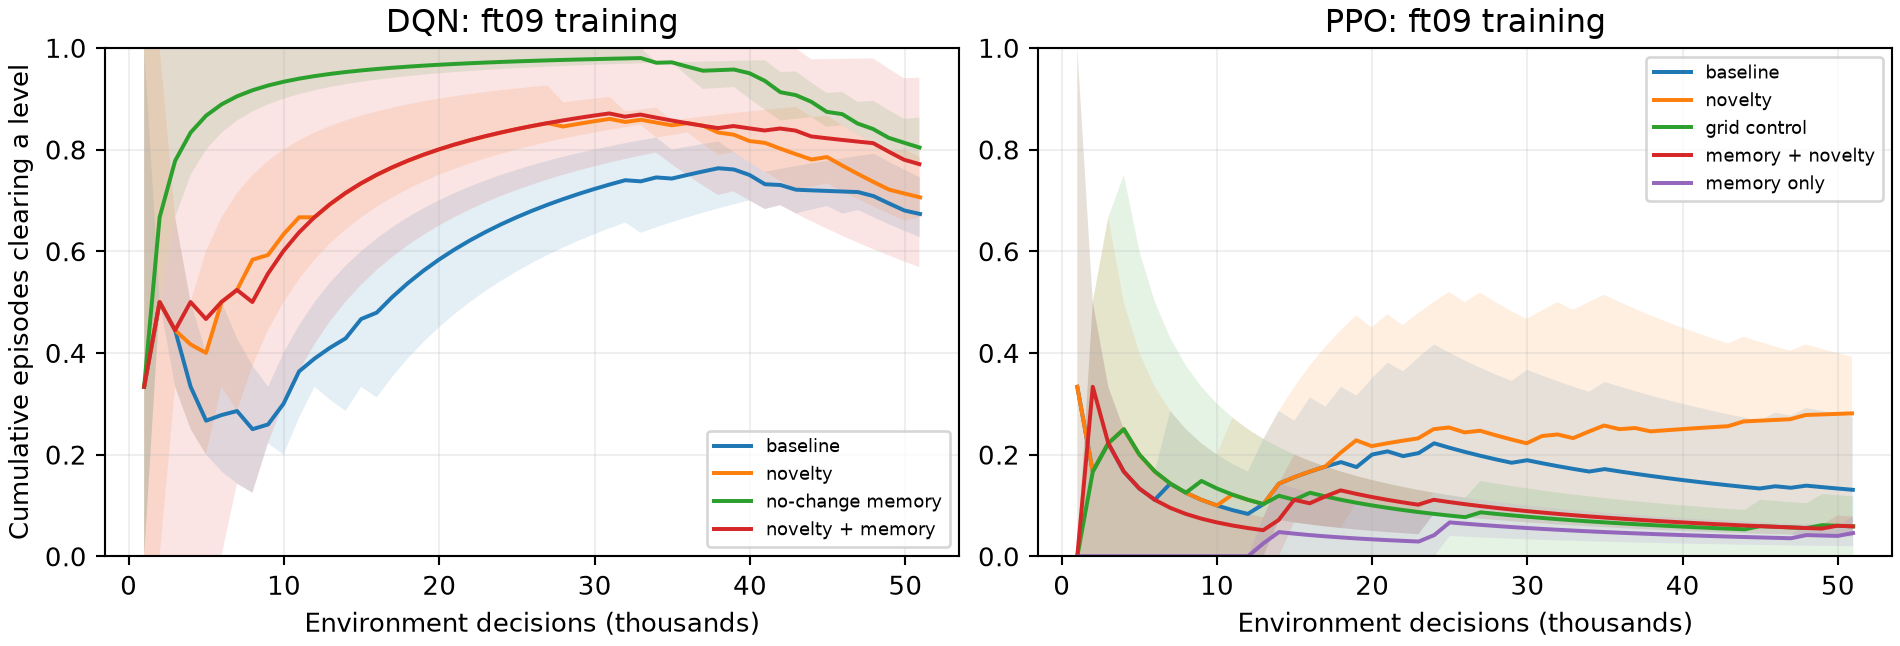
\includegraphics[width=\linewidth]{images/learning_curves.png}
\caption{Cumulative training episodes clearing a level on ft09 against decisions. Lines are means over three training seeds; shaded regions span their minimum and maximum. These curves show exploratory training behaviour, not frozen evaluation. DQN training includes epsilon exploration; PPO novelty conditions also receive intrinsic reward.}
\label{fig:learning}
\end{figure}

\subsection{Comparison, variability and cost}
On ft09, DQN with evaluation exploration exceeds both the sampled PPO baseline and pooled novelty PPO (Table~\ref{tab:results}). This is a narrow development comparison, not evidence of general superiority: the evaluation policies differ and epsilon was chosen on development data. No DQN condition completes a level on the other three development games. PPO completes none on dc22 and m0r0; memory-only PPO completes one g50t level in 60 rollouts, and all other g50t conditions complete none. Single successes do not show reliable adaptation.

All PPO greedy evaluations complete zero levels. Earlier greedy evaluations of improved DQN on ft09 contain one episode per seed, against 20 for stochastic evaluations, so greedy and stochastic rates cannot be compared with equal precision. Every development episode uses its full 1,000-action budget because no game is won. Figure~\ref{fig:learning} shows training-time progress, which is stronger than the frozen-policy results.

\begin{table}[t]
\centering
\caption{ARC-AGI-3 RHAE score (\%), computed locally with the published methodology \citep{arc2026} and the per-level human baselines published with each game version (ft09-0d8bbf25, dc22-fdcac232, g50t-5849a774, m0r0-492f87ba, cd82-fb555c5d, tr87-cd924810, vc33-5430563c). Seed columns are ft09 means over 20 episodes, followed by their mean and standard deviation across seeds; Dev.\ is the mean over the four development games; Held-out is the mean over cd82, tr87 and vc33. Evaluation policies match Table~\ref{tab:results}. -- : not evaluated.}
\setlength{\tabcolsep}{3pt}\small
\begin{tabular}{lrrrrrr}
\toprule & \multicolumn{4}{c}{ft09} & & \\
\cmidrule(lr){2-5} Condition & Seed 0 & Seed 1 & Seed 2 & Mean $\pm$ SD & Dev. & Held-out \\
\midrule Random reference &0.005&0.016&0.019&0.013 $\pm$ 0.008&0.003&--\\
DQN baseline &0.070&0.969&0.035&0.358 $\pm$ 0.529&0.090&0.003\\
DQN novelty &0.044&0.001&0.014&0.019 $\pm$ 0.022&0.005&0.000\\
DQN no-change memory &0.021&0.173&0.018&0.071 $\pm$ 0.089&0.018&0.000\\
DQN novelty + memory &0.713&0.280&0.090&0.361 $\pm$ 0.319&--&--\\
DQN baseline + evaluation-time memory &0.339&1.259&0.018&0.538 $\pm$ 0.644&--&--\\
PPO baseline, grid 8 &0.001&0.000&0.014&0.005 $\pm$ 0.008&0.001&0.000\\
PPO novelty, grid 8 &0.003&0.011&0.869&0.294 $\pm$ 0.498&0.074&0.000\\
PPO novelty, grid 16 control &0.000&0.037&0.001&0.012 $\pm$ 0.021&0.003&--\\
PPO memory + novelty, grid 16 &0.002&0.007&0.003&0.004 $\pm$ 0.003&0.001&0.000\\
PPO memory only, grid 16 &0.051&0.000&0.005&0.019 $\pm$ 0.028&0.005&--\\
\bottomrule
\end{tabular}
\label{tab:rhae}
\end{table}

Table~\ref{tab:rhae} applies the published RHAE formula to our recorded episodes. RHAE rewards efficiency as well as completion. A level solved in $a$ actions scores $\min(1.15,(h/a)^2)$, where $h$ is the human baseline, and a game score weights level $l$ by $l$ over all of the game's levels. Because ft09 has six levels, clearing only level one is worth at most 5.5\% of the game. Successful episodes clear it in a median of 372 actions (DQN baseline) and 232 actions (novelty PPO), against a human baseline of 43, so even they score little. RHAE ranks the conditions in nearly the same order as completion counts. The best pooled ft09 score is 0.36\% (DQN baseline and combined DQN), or 0.54\% with evaluation-time memory. RHAE also widens the gap between the best agents and random play: random clears ft09 level one in 15/60 episodes but needs a median of 529 actions, scoring 0.013\%. Every condition scores below 0.01\% on the held-out games. These are local scores on public games, not Kaggle leaderboard scores. Our counts exclude the initial reset. Including it would add one action to the first-level completion count and slightly reduce the nonzero scores. These values reconstruct scores from logs; they are not scores returned by the official gateway.

Across 12 training runs per stage, DQN baseline, novelty and memory take 7.34, 7.17 and 7.04 hours, with about 609,000 decisions each. Combined DQN adds 1.81 hours for three ft09 runs (152,726 decisions). PPO baseline and novelty take 1.26 and 1.38 hours; grid control, memory plus novelty and memory only take 1.53, 1.80 and 1.80 hours. These figures exclude evaluation, smoke tests and failed attempts. Evaluation cost is reported separately. All frozen evaluation, development and held-out together, took 0.85 hours for DQN (798 episodes) and 3.58 hours for PPO (2,295 episodes, including greedy diagnostics): about 3.8 and 5.6 seconds per episode. The held-out evaluation alone took 20 minutes. In the evaluation CSVs, wall time is cumulative, so a file's cost is its final value. CPU DQN against GPU PPO remains a hardware confound.

\section{Behavioural diagnosis and final transfer}
A sampled novelty-PPO trajectory clears ft09 level one and then makes 690 ineffective decisions. Read-only inspection of the development game shows that the original lattice reaches all eight first-level tiles but none of the 13 second-level tiles. A 16-by-16 lattice reaches all 13. With the original action set, level two cannot be solved whatever the policy learns. Coverage is necessary but not sufficient: the finer-grid control lowers first-level completion relative to novelty with grid 8. A larger exploration space is a plausible cause, but this experiment does not isolate it.

\begin{figure}[t]
\centering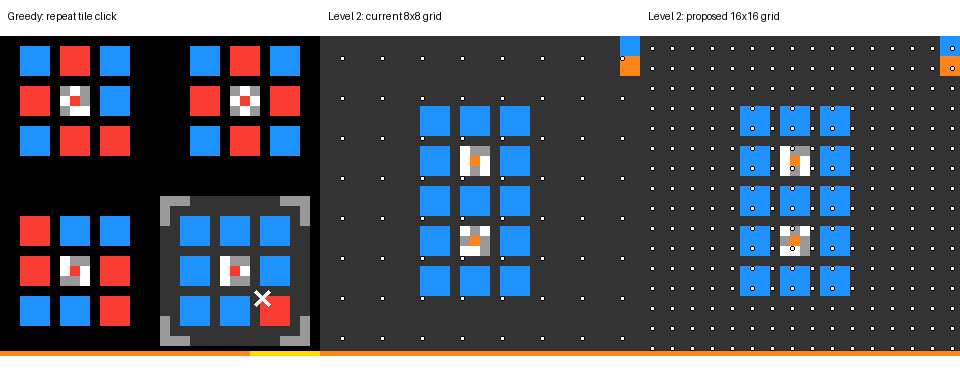
\includegraphics[width=\linewidth]{images/diagnostic.png}
\caption{Development diagnosis from recorded play: a repeated tile click changes pixels without solving the puzzle (left). The second-level puzzle has no reachable tile under the 8-by-8 lattice (centre); the 16-by-16 lattice reaches its tiles (right). Game source and state are used for this interpretation only, never as policy input.}
\label{fig:diagnostic}
\end{figure}

The greedy agent's repeated colour toggling also shows why a no-change mask cannot catch every unproductive cycle: a screen can change without making progress. A sequence model could capture longer dependencies, but no architecture can select an unreachable action or guarantee discovery from sparse success. The natural next experiment compares reachable action abstractions and longer action-conditioned memory under matched exploration budgets.

The final transfer evaluation takes all three ft09-trained seeds of each
algorithm's baseline, novelty and final memory stage (DQN no-change memory;
PPO memory + novelty) and runs them unchanged on
cd82, tr87 and vc33. Each checkpoint plays five rollouts per game, with sampling
seeds 100--104 and the same 1,000-action budget: 270 episodes across six stages.
Five rollouts rather than 20 keep the evaluation cost manageable while retaining
all three training seeds. No held-out outcome influenced model selection or
parameters. This tests transfer from a single training game, not online
adaptation or multi-game training.

All PPO stages and both improved DQN stages complete zero levels on all three
held-out games. DQN baseline seed 1 completes one tr87 level in one of five
rollouts (one of 15 pooled baseline rollouts on tr87); its other seeds complete
none. No agent wins a game, and every episode uses its full action budget. The
single completion does not establish generalisation. Development success on one
game therefore gives little assurance of transfer to a new puzzle under this
protocol. Per-seed results and the frozen protocol are in the evidence folder.


\section{Submission, limitations and conclusion}
We provide one notebook for each of the four DQN conditions and five PPO conditions. Each notebook embeds its inference code and loads exported NumPy weights from an attached model dataset; exported outputs match the original PyTorch networks. All notebooks use the official Agent interface and require a GPU. Kaggle must use its own Linux environment and installed PyTorch, not the Windows CUDA wheel used for training. Local CUDA inference and agent-loop checks passed; the Kaggle offline installation and live gateway remain untested. Models are applied unchanged to every game, with no routing by game identity.

The nominated entry is DQN baseline seed 1 with epsilon 0.3, chosen on development performance before transfer results were seen. PPO novelty seed 2 is the principal PPO alternative. Both use the 8-by-8 grid and so keep its reachability limitation. The nominee is one selected checkpoint, not the three-seed average, and its 20/20 development result carries selection bias. No parameters adapt during evaluation. Visual, no-change and action memories reset between games, and nothing is shared across games.

Development-game source and state were inspected to diagnose coverage and trajectories. Training and inference use only public observations, legal actions and the agent's past actions; no held-out source, solution or game-specific action script is used. One PPO run failed with a host-memory error and was restarted; its partial outputs are excluded. The conclusions are limited by missing early configurations, unequal hardware, selection on development games, small transfer samples and local rather than Kaggle scoring.

Our contribution is a reproducible two-algorithm investigation with tested interventions, several of them unsuccessful. Exploration produces useful first-level behaviour, but completion varies sharply by seed and does not extend to full games. Representation checks and trajectory inspection explain failures that aggregate rewards hide. The results call for more careful action design and controlled exploration studies; neither final agent solves ARC-AGI-3.

\section*{Contributions and AI assistance}
Nathan Le Roux: DQN implementation and experiments. Tafara Chibanda: PPO development, experimental iteration and submission integration. Samuel Snyman and Joshua Snyman: setup and documentation. Claude assisted with the initial scaffold; Codex assisted with implementation, debugging, analysis, packaging and writing. The authors are responsible for the code, results and attribution. Reused resources are PyTorch, NumPy, Gymnasium, arc-agi, arcengine and the official competition starter and framework. No external pretrained model is used.

\begin{thebibliography}{99}
\bibitem[ARC Prize(2026)]{arc2026} ARC Prize. ARC-AGI-3 competition documentation and official starter. \url{https://docs.arcprize.org/arc-prize-2026}; \url{https://github.com/arcprize/ARC-AGI-3-Kaggle-Starter}. Accessed 27 October 2026.
\bibitem[ARC Prize Foundation(2026)]{arcagi3} ARC Prize Foundation. ARC-AGI-3: A new challenge for frontier agentic intelligence. arXiv:2603.24621, 2026.
\bibitem[Bellemare et al.(2016)]{bellemare2016} Marc G. Bellemare, Sriram Srinivasan, Georg Ostrovski, Tom Schaul, David Saxton and R\'emi Munos. Unifying count-based exploration and intrinsic motivation. \emph{NeurIPS}, 2016. arXiv:1606.01868.
\bibitem[Burda et al.(2019)]{burda2019} Yuri Burda, Harrison Edwards, Amos Storkey and Oleg Klimov. Exploration by random network distillation. \emph{ICLR}, 2019. arXiv:1810.12894.
\bibitem[Harris et al.(2020)]{harris2020} Charles R. Harris et al. Array programming with NumPy. \emph{Nature}, 585:357--362, 2020.
\bibitem[Kingma and Ba(2015)]{kingma2015} Diederik P. Kingma and Jimmy Ba. Adam: A method for stochastic optimization. \emph{ICLR}, 2015. arXiv:1412.6980.
\bibitem[Mnih et al.(2015)]{mnih2015} Volodymyr Mnih et al. Human-level control through deep reinforcement learning. \emph{Nature}, 518:529--533, 2015. \url{https://doi.org/10.1038/nature14236}.
\bibitem[Paszke et al.(2019)]{paszke2019} Adam Paszke et al. PyTorch: An imperative style, high-performance deep learning library. \emph{NeurIPS}, 2019.
\bibitem[Pathak et al.(2017)]{pathak2017} Deepak Pathak, Pulkit Agrawal, Alexei A. Efros and Trevor Darrell. Curiosity-driven exploration by self-supervised prediction. \emph{ICML}, 2017.
\bibitem[Schulman et al.(2016)]{schulman2016} John Schulman et al. High-Dimensional Continuous Control Using Generalized Advantage Estimation. ICLR, 2016. arXiv:1506.02438.
\bibitem[Schulman et al.(2017)]{schulman2017} John Schulman, Filip Wolski, Prafulla Dhariwal, Alec Radford and Oleg Klimov. Proximal Policy Optimization Algorithms. arXiv:1707.06347, 2017.
\bibitem[Strehl and Littman(2008)]{strehl2008} Alexander L. Strehl and Michael L. Littman. An analysis of model-based interval estimation for Markov decision processes. \emph{Journal of Computer and System Sciences}, 74(8):1309--1331, 2008.
\bibitem[Towers et al.(2024)]{towers2024} Mark Towers et al. Gymnasium: A standard interface for reinforcement learning environments. arXiv:2407.17032, 2024.
\end{thebibliography}
\end{document}
